\documentclass{llncs}
\usepackage{lipsum}

\usepackage{listings}
\usepackage{color}
\usepackage{setspace}

\usepackage{graphicx}

% \newcommand{\ts}{\textsuperscript}
% \usepackage{minted}

\definecolor{Code}{rgb}{0,0,0}
\definecolor{Decorators}{rgb}{0.5,0.5,0.5}
\definecolor{Numbers}{rgb}{0.5,0,0}
\definecolor{MatchingBrackets}{rgb}{0.25,0.5,0.5}
\definecolor{Keywords}{rgb}{0,0,1}
\definecolor{self}{rgb}{0,0,0}
\definecolor{Strings}{rgb}{0,0.63,0}
\definecolor{Comments}{rgb}{0,0.63,1}
\definecolor{Backquotes}{rgb}{0,0,0}
\definecolor{Classname}{rgb}{0,0,0}
\definecolor{FunctionName}{rgb}{0,0,0}
\definecolor{Operators}{rgb}{0,0,0}
\definecolor{Background}{rgb}{0.98,0.98,0.98}


\begin{document}
\title{MarketMaker:\\Multi-armed Bandits inspired trading algorithm}
\subtitle{Bristol Stock Exchange extension\\[1em]\today}
\author{Kacper \textbf{Sokol}---ks1591---45684}
\institute{Department of Computer Science,\\
  University of Bristol,\\
  Bristol, BS8 1UB\\
  \email{k.sokol.2011@my.bristol.ac.uk}}
%
\maketitle
%

\begin{abstract}
This paper introduces trading algorithm for \emph{Bristol Stock Exchange}%
\footnote{\url{https://github.com/davecliff/BristolStockExchange}} %
which is inspired by \emph{Multi-armed Bandits} approach to \emph{exploration vs.\ exploitation} problem. Presented here algorithm is a wrapper for arbitrary trading agent. It uses aforementioned model to determine the best possible strategy for current trading session by adapting to opponents configuration.
\end{abstract}
\keywords{Bristol, Stock, Exchange, Multi-armed, Bandits, Trading, Algorithm}

\section{Introduction}
Bristol Stock Exchange(BSE) is a simple and minimal simulation of \emph{limit order book}(LOB) financial exchange with single tradable security. In the market any trader can issue an order, where each new order replaces the old one. It also assumes zero latency in communication between the traders and the exchange and that information about newly issued orders is distributed among agents before the next order can be issued.\\

Designed algorithm trades on BSE using sub-traders---it is a wrapper for generic trading algorithm. In this study, used sub-traders are the one contained by default in BSE source code, but this is easily modifiable. Each order is issued with sub-trader considered for given moment as the most profitable. The choice which trader to use is governed by simplistic implementation of \emph{Multi-armed Bandits}(MABs) algorithm.\\
Presented here trader differs from implemented in BSE agents as it is a Market-Maker: it trades with its own money and decides what and when to trade. On contrary, BSE own traders are \emph{sales trader} who receive external orders and make profit from the price difference they can make.\\

To the best of my knowledge, presented here approach is first of its kind and has not been described or tested up. The source code of the algorithm is available both: in the \emph{\appendixname} at the end of this paper (\emph{Listing~\ref{lst:MABmm}}), and on-line at: \url{https://github.com/So-Cool/MABtrader}.\\

\section{Methodology}
The stock exchange market is highly complex system, which dynamics is governed by supply and demand. Many different traders with wide range of strategies issue orders to trade securities with highest possible margin. The best possible agent should beat the competition by adapting to constantly changing market situation. To address this issue I decided to use Multi-armed Bandits framework with \emph{Upper Confidence Bound}(UCB) approach.\\

The decision when and what order to issue is based on two concepts: $k-$\texttt{lag} ($10-$\texttt{lag}) of recent \emph{best} and \emph{worst} of \emph{bids} and \emph{asks} on the LOB, and \emph{critical point}. The first one identifies actual trend on the market to decide on the price and type of order to make. The latter identifies approaching market closure---10\% of session time left---to disable buying and short-selling (if allowed) and get rid of all possessed assets.\\
Chosen approach, does not require complex price analysis mechanism to maximise a profit of a trade as employed sub-traders work is to maximise their commission which in this case flows to Market-Maker's pocket. Used sub-traders while given a price paid for asset will enforce this price as minimal and do their best to maximise profit.\\
The agent is capable of short-selling and has a predefined cap on number of possessed assets. For presented in this paper experiment it is allowed to collect up to $1$ assets, and both: experiments with enabled and disabled short selling were carried out.\\

To test designed \emph{MarketMaker} \textbf{22751} trading round were carried out each consisting of 33 traders: 16 buyers and 16 sellers of types Giveaway, Shaver, ZIC, and ZIP with the ratio of the four types of traders being systematically varied across all possible non-zero values with 50 independent trials for each specification ratio. The one additional trader to this compilation was designed MAB MarketMaker.

\subsection{Order issuing}
Order issuing in presented trader is based on well known tool for time-series analysis called $k-$\texttt{lag}: it inspects the difference between current and $k$\ts{th} most recent prices at the market. It is used by the trader to calculate \emph{best} price trend of the LOB's \emph{bids} and \emph{asks}. Until the corresponding trend was rising (falling) the order was not issued. Once the trend has faltered the agent started making and offers: it bought assets based on minimum price of recent best bids and its sell prices, and sold assets based on maximum of best ask and its buy price.\\

The task of working on margins is left to employed sub-traders. Each of them is sales trader and its task is to work out best possible margin on given price. This allows the agent to issue order with at least paid price (or more depending on market situation) and collect overhead earn by sub-trader if order is executed.\\
For the experiments presented below if the robot reaches its assets cap it is only allowed to sell or buy-back (if previously short-sold). If the limit is not reached the robot is allowed to decide whether to buy(-back) or (short-)sell based on speed of change in price trend.\\

The robot is capable of short-selling but due to BSE design it was disabled for the experiments. The main issue was that once the trader issued a \emph{bid} or \emph{ask} it had to continue issuing this type of order until it offer was crossed by other trader. Otherwise there is a possibility of crossing one's own offer or other robot. Hence, without substantial changes to BSE design interchangeable orders could not be issued.\\

When the end of trading session is approaching the the trader clears all its assets. If there exist short-sold items it will buy them back; if it holds any asset it will sell it; if it does not posses anything buying and selling will be disabled.

\subsection{Sub-trader choosing with MAB}
The design of discussed trader is inspired by gaining in popularity in recent years framework for testing hypothesis. Multi-armed bandits are taking place of \emph{A-B testing} as they allow for dynamic change of environmental set-up and not only data collection for later analysis.\\
The main concept behind them is simply row of slot machines each yielding some reward distributed according to some unknown distribution. Once the armed was pulled the machine gives us reward which then can be used to better estimate the distribution underlying this reward. The more we play given machine the better we understand its reward mechanism.\\
The main problem with this setting is balancing \emph{exploration} and \emph{exploitation} to achieve optimal long term reward. The exploration is roughly speaking using under-discovered machines to learn more about the environment and exploitation is using current knowledge to play machine considered as most rewarding to increase overall reward.\\
Multi-armed Bandits is well documented by~\cite{berry+firstedt,gittins+glazebrook+weber} problem with some simple tackling this vast problem. MABs are well known technique in on-line adversing and are used to maximise the click-through rate by arranging ads in best suited places for given customer by companies such as Google~\cite{AYPSze12,ASMB:ASMB874}, LinkedIn~\cite{Tang:2013:AAF:2505515.2514700}, Microsoft~\cite{graepel2010web}, Yahoo~\cite{Li:2010:CAP:1772690.1772758}.\\

In trader context I adapted MAB technique where traders are arms in the machine; reward is the profit made by trader on given order; and exploration vs. exploitation is discovering potential associated with each trader in current market.\\
The approach to solve this MAB problem is \emph{Upper Confidence Bound}(UCB)~\cite{white2012bandit} which is simple yet powerful technique to find optimal solution. Furthermore, it prevents ``\emph{sticking}'' i.e.\ using arm (trader) that is currently best but too little is known about other arms(traders) to  have strong evidence of its superiority.\\

Application of MAB in trader creates possibility of probabilistic choices based on current market structure. It does not require complex Bayesian approach: collecting enormous amount of data would be impractical. Furthermore it does not require to construct complex decision if-else model analysing current market structure to choose appropriate to use trader. Both this feature of chosen solution give great flexibility and adaptability.\\

Presented trader is a simple wrapper for traders compatible with BSE. It calls appropriate methods at each of them updating their internal variables and issuing them orders. Once single trader is chosen for given round its order is collected and submitted to the exchange as presented trader's order.\\
The algorithm ensures that every sub-trader was tried at least once to collect the reward (earnings on trade) and be able to calculate its potential in the market. Then by calculating UCB on rewards plus the uncertainty parameter of solution it chooses the best solution for current market. The uncertainty parameter ensures exploration of other solutions outside of the best scoring and acts a a changing lever if current sub-trader begins to under-perform in comparison with other available sub-traders until the reward is maximised again.\\

In carried out experiments the opponents of MAB trader were the same as employed sub-traders. This situation may result in advantageous behaviour of presented trader as it knows the algorithms of competition.

\section{Results}
% One / Multiple in the MArket # try LONGER SESSIONS to allow it to learn

\begin{table}[ht]
  \centering
  \begin{tabular}{ p{5em} | p{5em}  p{5em}  p{5em} }
    name & mean & median & standard deviation \\
    \hline
    GWY  & $130.0$ &$ 130.0$ &$ 24.4$ \\
    MAB  & $12.7 $& $16.0 $& $37.9$ \\
    SHVR & $112.1$& $112.0 $& $13.2$\\
    ZIC  & $89.6 $& $87.0 $& $16.0$\\
    ZIP  & $130.3$ &$ 129.8$ & $12.2$
  \end{tabular}
  \vspace*{1em}
  \caption{Basic statistics for traders.\label{tab:stats}}
\end{table}

\begin{figure}[ht]
  \centering
  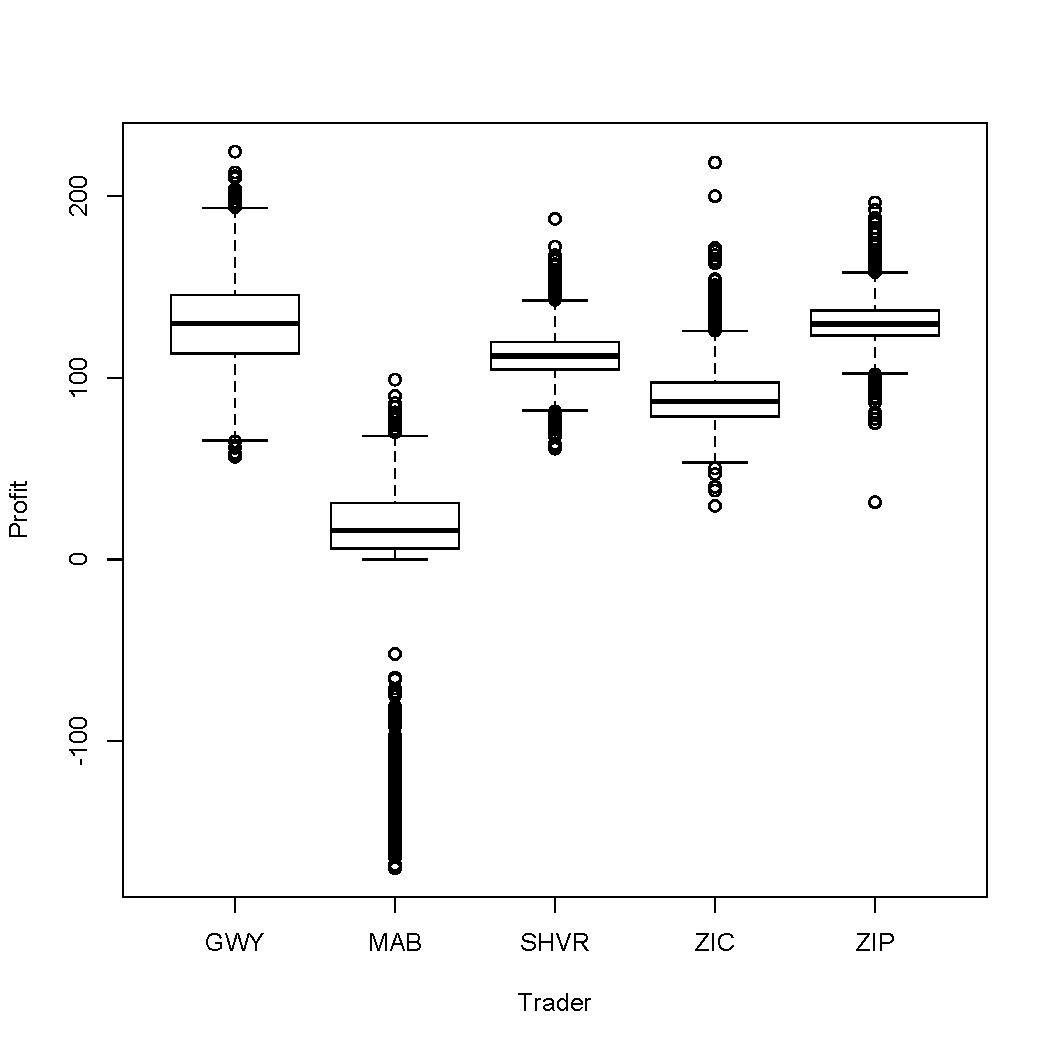
\includegraphics[width=.7\textwidth]{fig/box.pdf}
  \caption{Box-plot of profits for all traders.\label{fig:box}}
\end{figure}

The negative profit visible for MAB traders is due to assets that were bought and couldn't be sold by the end of market session.\\

\begin{figure}[ht]
  \centering
  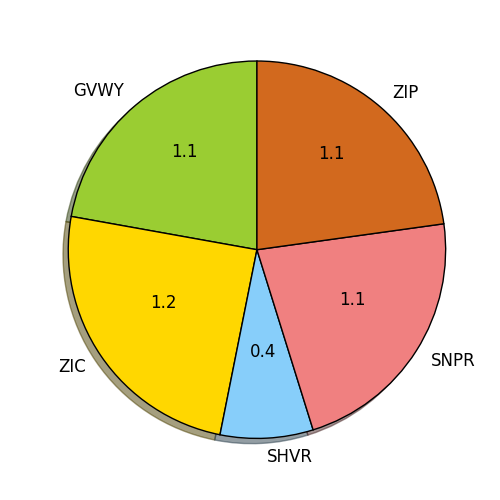
\includegraphics[width=.5\textwidth]{fig/pie.png}
  \caption{Sub-traders used by MAB MArketMaker.\label{fig:MABalgo}}
\end{figure}

\begin{table}[ht]
  \centering
  \begin{tabular}{ p{5em} | p{5em} p{5em} p{5em} p{5em} }
         &GWY    &MAB    &SHVR   &ZIC   \\
    \hline
    MAB  &$<2e-16 $&$-      $&$-      $&$-     $\\
    SHVR &$<2e-16 $&$<2e-16 $&$-      $&$-     $\\
    ZIC  &$<2e-16 $&$<2e-16 $&$<2e-16 $&$-     $\\
    ZIP  &$0.28   $&$<2e-16 $&$<2e-16 $&$<2e-16$
  \end{tabular}
  \vspace*{1em}
  \caption{Results of Wilcoxon-Mann-Whitney U Test.\label{tab:wilcox}}
\end{table}

Average MAB trades per game: \textbf{4.78}\\


Kruskal-Wallis Test\\
robust-rank corelation test

\section{Discussion}
Presented in this paper solution discusses novel---probabilistic---approach to trading agents inspired by Multi-armed Bandits. As stock exchange markets contains vast number of independent and self-centred agents it is important to ensure that produced trader can quickly adapt to its environment.\\
The key strength of my solution is modularity of used sub-traders. It is possible to use relatively large number of them, each adapted to different market structure. Without explicitly specifying rules governing use of particular trader, UCB will try each solution and based on earned amount it will converge to most profitable one. In case of sudden market shift it will try another traders to check for improvements of current strategy.\\

Based on presented above statistical analysis designed algorithm performs relatively bad in comparison with all other algorithms used in experiment. It only detects a few possibilities to earn money (\textbf{4.75} trades per session). Furthermore, the average number of trades made per sessions undermines the concept of using Multi-armed Bandits as sub-trader choosing mechanisms. Almost uniform sub-traders use indicates that full potential of MAB is not used. The longer sessions and more trading opportunities is needed to allow MAB algorithm to learn and use the best strategy for current market structure.\\


\section{Conclusion}
Used approach is novel and the paper presents only rough framework how to use it. There is still lot of work to be done and research to be carried out to understand use of Multi-armed Bandits in trading algorithms.\\

This study engages only use of predefined in BSE traders. Presented here framework can be easily generalised to use more complex and diversified sub-traders covering wider range of possible market situations. The next viable goal extending this study would be to employ more sub-traders and check the performance of proposed solution.\\
Furthermore, another study is needed to check the behaviour of trader when it can change its status from selling to buying without making a transaction. Enabling multiple orders and short-selling might also be worth inspecting. Also interesting should be deploying multiple MAB MArketMakers and see how they interact.\\
Also another study is needed inspecting behaviour of MAB trader where used sub-traders differ from other strategies used by other agents in the market.\\
Finally, as MAB strategies show their full potential in long run experiments another study should be carried out with longer trading sessions.


\vfill
\bibliographystyle{plain}
\bibliography{ref}

\newpage
% \begin{appendices}
\section*{\appendixname: MAB MarketMaker source code\label{app:MABmm}}

% \inputminted[
% frame=lines,
% framesep=2mm,
% baselinestretch=1.2,
% fontsize=\footnotesize,
% linenos
% ]{python}{../code/marketMaker.py}

\lstset{
captionpos=b,
breaklines=true,
caption=MAB MarketMaker source code,
label=lst:MABmm,
%
numbers=left,
numberstyle=\footnotesize,
numbersep=1em,
xleftmargin=1em,
framextopmargin=2em,
framexbottommargin=2em,
showspaces=false,
showtabs=false,
showstringspaces=false,
frame=l,
tabsize=4,
% Basic
basicstyle=\ttfamily\small\setstretch{1},
backgroundcolor=\color{Background},
language=Python,
% Comments
commentstyle=\color{Comments}\slshape,
% Strings
stringstyle=\color{Strings},
morecomment=[s][\color{Strings}]{"""}{"""},
morecomment=[s][\color{Strings}]{'''}{'''},
% keywords
morekeywords={import,from,class,def,for,while,if,is,in,elif,else,not,and,or,print,break,continue,return,True,False,None,access,as,,del,except,exec,finally,global,import,lambda,pass,print,raise,try,assert},
keywordstyle={\color{Keywords}\bfseries},
% additional keywords
morekeywords={[2]@invariant},
keywordstyle={[2]\color{Decorators}\slshape},
emph={self},
emphstyle={\color{self}\slshape},
% 
}\lstinputlisting{../code/marketMaker.py}


\end{document}
